\documentclass[fleqn]{report}
\usepackage{geometry}
\usepackage{amssymb}
\usepackage{fancyhdr}
\usepackage{multicol}
\usepackage{blindtext}
\usepackage{color}
\usepackage[fontsize=16pt]{fontsize}
\usepackage{lipsum}
\usepackage{pgfplots}
\usepackage{physics}
\usepackage{mathtools}
\usepackage[makeroom]{cancel}
\usepackage{ulem}

\setlength{\columnsep}{1cm}
\addtolength{\jot}{0.1cm}
\def\columnseprulecolor{\color{blue}}
\date{Spring 2025}

\newcommand{\textoverline}[1]{$\overline{\mbox{#1}}$}

\newcommand{\hp}{\hspace{1cm}}

\newcommand{\const}{\textrm{const}}

\newcommand{\del}{\partial}

\newcommand{\pdif}[2]{ \frac{\partial #1}{ \partial #2} }

\newcommand{\pderiv}[1]{ \frac{\partial}{ \partial #1} }

\newcommand{\comment}[1]{}

\newcommand{\equations} [1] {
\begin{gather*}
#1
\end{gather*}
}

\newcommand{\numequations} [1] {
\begin{gather}
#1
\end{gather}
}

\newcommand{\twovec}[2]{ 
\begin{pmatrix}
#1 \\ 
#2
\end{pmatrix}
}

\title{CS 482}
\author{Aiden Sirotkine}

\begin{document}

\graphicspath{ {../Images/} }
\pagestyle{fancy}
\maketitle
\tableofcontents
\clearpage

\chapter{CS 482}
This'll be an interesting class lets hope I can figure out stats.

\begin{itemize}
    \item 
    building complex models 
    \item 
    algorithmic randomness 
    \item 
    statistically analyzing data
\end{itemize}

Chuck data into a black box of modelling code and get result data out. 

Simulations give the most realistic answers for complex systems that cannot be 
linearly solved. 

Simulation is only good for basically unsolvable problems. 

\chapter{Terminology}

\section{System}
A collection of \textit{entities} that interact with a common 
purpose according to sets of \textit{laws} and \textit{policies}

example: a store, airport terminal, etc. \hp most things 

\section{Entities}
The components/objects that define a system

Physical or Logical objects 

Temporary or Permanent 

\section{Attributes}
The traits that define an entity 

static or dynamic

qualitative or quantitative 

A cashier in a store :
\begin{itemize}
    \item 
    has a high school diploma (static, qualitative)
    \item 
    has an IQ of 104 (static, quantitative)
    \item 
    can be busy or idle (dynamic, qualitative)
    \item 
    can process customers at a rate from 6/hour to 20/hour (dynamic, quantitative)
\end{itemize}

\section{Entity-Attribute Hierarchy}
determines the level of detail in the simulation 
\begin{itemize}
    \item 
    Regional Plants 
    \item 
    Production Lines 
    \item 
    Work Areas 
    \item 
    Machines, Tools, Operators 
\end{itemize}

The \textit{level of detail} in the simulation model 
is set by the entity/attribute hierarchy boundary, 
which is determined by the \textit{objectives of the study}. 

Attributes become entities if you want more detail in a system 

The boundary between attribute/entity determines the level of detail 
in the simulation. 

\section{Laws and Policies}
Both Laws and Policies govern the behavior of the system, but Laws cannot 
be changed while Policies can be changed. 

Laws are followed, Policies are set. 

\section{Model}
The thing that we're trying to do in this class 

A simplification of a system 

there are many ways to model a system 
\begin{enumerate}
    \item 
    Events List 
    \item 
    Difference Equations 
    \item 
    Markov Chains 
\end{enumerate}

\subsection{State Space}
A Collection of variables that represent and measure the condition of the system 
(busy, idle, broken, etc.)

The state space is the \textit{film} for a photo snapshot of a system.

\section{Event}
An instant of time when one of the following occurs 

\begin{itemize}
    \item
    the state(s) change(s)
    \item 
    other events are caused (scheduled) or prevented (cancelled)
    (i.e. other states change)
    \item 
    data is collecte dand statistics may be compiled 
    (based on or uses states)
\end{itemize}

examples:
\begin{itemize}
    \item
    a part arrives 
    \item
    A machine starts or stops or breaks down 
    \item
    The end of day of operation 
\end{itemize}

\section{Process}
An indexed set of states of events 

Let $N_t$ be hte number of customers in the system at time $t$ 

Let $B_j$ be a $0-1$ indicator of whether or not that $j$th customer does 
or doesn't get on hold. 

\section{Discrete-Event Simulation}
A model where the state $S$ changes at \textit{discrete} points in time 

what/when/how/what impact of changes 

\section{Single Server Queue}
$\lambda$ is the rate at which parts arrive 

$\mu$ is the rate at wich the server can process parts 

Number in system = number in queue + number in service. 

events schedule other events.

\section{Building Simulation Models}
\begin{itemize}
    \item 
    define states 
    \item 
    identify when and how the state change 
    \item 
    define events 
    \item 
    define initialization 
\end{itemize}

\begin{itemize}
    \item
    ALL simulation models have an initialization event. 
    \item
    assume a random number generator is available 
    \item
    a new random variable value must be generated each time a 
    random variable is used or called 
    \item
    arrival events schedule more arrival events (self-generating)
\end{itemize}

\subsection{When executing an event:}

\begin{itemize}
    \item
    State changes occur first 
    \item
    Events scheduled or cancelled occur second 
\end{itemize}

Once you have all of the states and changes and whatever, coding 
the simulation itself is not actually that hard. 
    
hop from most recent event to most recent event until done, 
changing the event queue as needed. 

\subsection{Dynamic Simulation}
\begin{itemize}
    \item
Events are scheduled and executed in \underline{time sequence}
    \item
States are changed as each event is executed 
    \item
Data can be colelcted as events to do stats and math stuff 
    \item
Know where to collect data and what type of data to collect. 
\end{itemize}


\section{Data Tracking}
\begin{itemize}
    \item
If we want to determine the customer waiting times in the systme, 
we need to record both the arrival time ARRTIME and the departure 
time DEPTIME. We can then calculate WAITINSYS = DEPTIME - ARRTIME
    \item
What we do is at an event, we also record data, 
    \item
So for example, when a customer arrives, we record the time in ARRTIME 
at the point of that event. 
    \item
You need to make sure that you have indexes for each arrival 
and exit so that you can correlate waiting times to entities. 
\end{itemize}

\section{Simulataneous Events}
\begin{itemize}
    \item
It doesn't happen super often but it does happen and we still have 
to do things sequentially 
    \item
For example, if we want to track the number of times the server becomes idle 
then if the server completes a task as a new customer arrives, we don't want 
the server to be open for $0$ seconds, so the simultaneity of the task 
actually makes a difference in things. 
    \item 
You can also randomize what events happen first and that might fix 
whatever issues might occur. 
    \item
Just be aware that it is an issue 
\end{itemize}

\section{Static Simulation Models}
\begin{itemize}
    \item 
Easier than dynamic models 
\item 
time is not really a factor 
\item 
Event lists are not needed (though can still be used)
\item 
Events are naturally sequential 
\end{itemize}

\section{Dice Game}
\begin{itemize}
    \item 
Is it better to roll 1 dice and try to get 5 twice, or roll 2 die and try 
to get 7, 11, or 12 three times in a row 
    \item 
can be done mathematically, but is trivial for a simulation 
    \item 
demonstration of how simulations can be useful over analytical mathing. 
\end{itemize}

\section{Buffer Allocation}
\begin{itemize}
    \item 
Consider a production line with 3 machines that flow into each other 
and process a certain amount of a parts per second
\item 
How large capacity of a buffer in between each machine do we need in order for machines 
to stop as little as possible?
\item 
Machines can be busy, idle, or blocked (meaning the buffer in front of it is 
full, so it cant make more stuff without overflowing)
\end{itemize}

\subsection{Policies}
\begin{itemize}
    \item 
    Parts are indistinguishable 
    \item 
    parts are first come first served 
    \item 
    Parts begin processing at a machine only if 
    there is space availbale in the buffer 
    \item 
    the buffer at the very end is infinity, so the last machine is on forever. 
\end{itemize}

\subsection{Events}
\begin{itemize}
    \item
    Arrival at Buffer
    \item 
    Exiting buffer 
    \item
    Arrival at Machine 
    \item 
    Exiting machine 
    \item 
    End of day 
\end{itemize}

\subsection{Priority}
When making simultaneous events, we have to figure out what happens first.

Does the machine pick up an item from the buffer first? Does the buffer 
decriment first? Does the previous machine try to add an item to 
the buffer first?

\section{Verification and Validation}
\begin{itemize}
    \item
    Does the simulation represent the real system?
    \item 
    Is the code correct 
\end{itemize}

\subsection{Techniques}
\begin{itemize}
    \item 
    Study the code carefully 
    \item 
    Make a trace through the simulation model to ensure 
    that even adn state changes are realistic 
    \item 
    Look at the simulation output. Doe sit 
    agree with known anlytic (theoretical) results?
    Does it work under certain restrictions?
    \item
    Fault/failure insertion testing:
    Put in bad data and see if it breaks correctly 
    \item 
    Set inputs at extreme values and see if the obvious happens 
    \item 
    Use historical data with known outputs and compare what the simulation yields.
\end{itemize}
\noindent 
Model validation tells us roughly how close our simulation is 
to the real system. 


\section{The Modeling Process}

With a real system you can create a conceptual model and then that gets 
 turned into a computer model that returns a bunch of data. 

 \subsection{Detail}

 If we add too much detail, we lose the big picture 
 and our simulation because obnoxious. 

 If we don't have enough detail, we lose accuracy. 

 Keep It Simple, Stupid

 If we're trying to make a restaurant, the number of customers 
 depends on the time of day. 

 The servers might or might not be distinguishable from each other 

 What are we measuring from the simulation?

 What foods are avaialable in the simulation?

 are there different table sizes?

 Start with the minimum amount of detail, and then go up from there. 

 Use the minimal amount of detail to answer your questions. 

 \section{Queuing Models}

 Seen in manufacturing, service, all sorts of stuff. 

 \subsection{M/M/1 Model}
 Markovian / Markovian / 1 server (single service queue)

 M/M queues are well studied and we have a good idea of how they work. 

\begin{itemize}
    \item
    M/M/1
    \item 
    M/M/c 
    \item 
    M/M/c Feedback 
    \item 
    M/M/1 Priority 
    \item 
    M/M/1/K
\end{itemize}

\subsection{Service Mechanims}
\begin{itemize}
    \item
    First in, First out 
    \item 
    Last in, First out 
    \item 
    random 
\end{itemize}

\subsection{Potential Measurements}
\begin{itemize}
    \item 
    average wait time per customer 
    \item 
    fraction of customers who wait more than 10 minutes 
    \item 
    average idle time per worker 
    \item 
    average number of idle workers 
\end{itemize}

\subsection{G/G/1}
Let $A_i$ be the inter-arrival time betwee ncustomers $i$ and $i+1$ 

Let $S_i$ be the servie time of customer $i$

Then $D_i$ is the delay time (waiting time in queue) of customer $i$

This type of queue ends up being governed by Lindsley's Equation 
\equations{
    D_i = max \{0, D_i + S_i - A_i\} 
    \hp 
    D_1 = 0
}
Only holds true for single server queuing system. 

\chapter{Simulation (Event) Graphs}
Graphical represenatation of entities, attributes, and state changes. 

Provides a universal representation for discrete-event simulation models 

IT'S NOT A FLOW CHART 

State changes occur at each node. 

\begin{itemize}
    \item 
    Scheduling edge 
    \item 
    Cancelling edge 
    \item 
    Self-scheduling event 
    \\
    Event A is scheduled every event A 
    \item 
    Simultaneous Sequential Event 
\end{itemize}

\section{Single Server Queue}
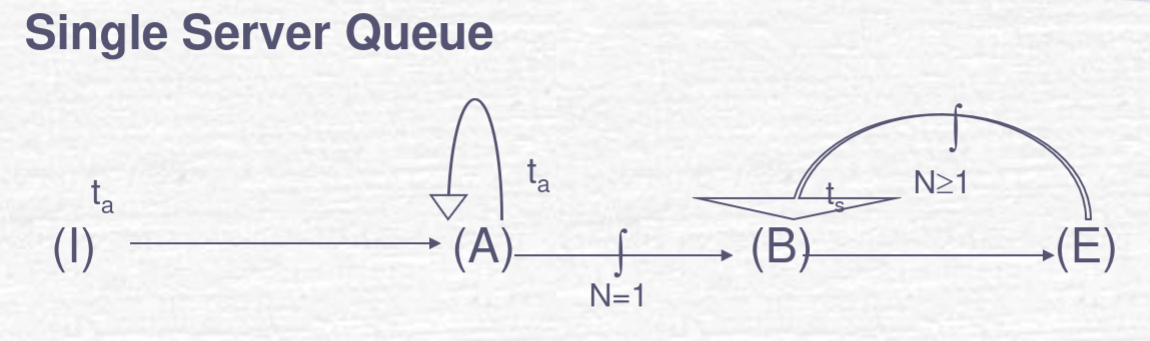
\includegraphics[width = 16cm, height = 5cm]{CS482.1.png}

Where $t_a$ is the time between arrivals and $t_s$ is the service time. 

It shows what is scheduled when and in what sequence. 

$\int$ means if a condition is met. 

The system is initialized, a things goes in the queue, if 
there is 1 server in the queue, begin service event, end service event, 
if there is someone in the queue, being servie event again. 

you can compress the graph a little more.

Every simulation's event graph can be made with 
1 initialization event and 1 node

sometimes simplifying a graph is very stupid because it gets rid of 
too much detail. 

\section{Edge Reduction}
An event node can be removed if there are no condition exit edges and oen of the 
following 
\begin{itemize}
    \item 
    zero delay times entering the edge
    \item 
    zero delay times exiting the edge
    \item 
    State changes are not associated with any edge conditions 
\end{itemize}

if $i)$ holds, then there can be condition exit edges 

reduced graphs are NOT isomorphic. The same system is being modeled but with a 
different level of detail.

\section{Variations of a Single Server Queue}
Consider multiple indistinguishable servers (bowling alley)

Number of idle servers is a state variable $S$ (number of idle servers)

Arrival is normal, begin service event is dependent on if $S > 0$,

end service event increments $S$.

Event $B$ (begin service) needs to have higher priority than events $E$ and $A$ 
to avoid "phantom" customers/servers. 

\subsection{Phanton Customer}
Supposed $A$ and $E$ begin at the same time.

If $E$ is executed first, then event $B$ is scheduled 

If $A$ is scheduled second, another $B$ is scheduled because that 
server is still considered as "idle"

if we execute $A$ first, we increment $Q$ by 1 and then schedule $B$ 

if $E$ is executed second, we increment $S$ and because $Q > 0$, we 
schedule another $B$ event for the same $A$.

This is why whenever $B$ is scheduled, $B$ needs to have priority.

\subsection{non-empty initial conditions}
Let $Q = q$ the initial number of people in the system.

consider a number $Q'$ Which is all the intitial people. 

We need to add a new event $P$ if there are people in the queue initially 

$P$ puts the initial people in the queue 1 by 1 until all the servers are 
full or there are no more people. 

$P$ needs to have higher priority than $B$ because we want everyone 
to be set to a server before any begin service queues begin. 

Consider $N$ the number of people in the system. 

\section{Batched Service/Arrivals}
$\beta$ is the batch of things in service and $\alpha$ is the number 
of customers that arrived. 

The server cannot serve an amount of customers under $\beta$

make sure that $B$ has a higher priority that $E$ and $A$ and then you'll
be set. 

It's pretty close to the same as a regular queue.

However, a busy period only begins as long as 

$\beta \leq N \leq \beta + \alpha$,
So the number in the system cannot be too too large or else we 
are already in a busy period. 

However, we can use a variable $L$ to determine whether or not we 
are in a busy period. 

if $N \geq \beta$ and $L = 1$ then the $B$ event begins, and 
if $E$ occurs and $N < \beta$, then $L$ goes to $1$ and it will 
wait for a large enough batch of customers. 

\section{Rework (Feedback)}
After $E$, if a certain event (rand(0, 1)) happens, then a REWORK 
event happens which queues another $E$ event after a certain amount of time. 

Because there's no begin service event, these simulations are clunky 

\subsection{Discard Rework}
There's a certain probability that a part gets thrown out after $E$. 

Nothing happens after the discard. 

\section{Limited Buffer Space}
page 127 

Consider an ENTER event. 

$N$ is number in the system. $M$ is the number of customers that arrived. 
$J$ is the number of customers that enter the queue.

$M - J$ is the number of people that get turned away 

Set event $E$ to have a higher priority than event $A$ so that 
the customers go through the system correctly and no one 
gets incorrectly turned away. 

\subsection{Indicator Functions}
You can use them instead of using the ENTER event. 

let $K$ be our buffer space 

if $N > K$, then we turn em away 

if $N \leq K$, then we add them to the queue. 

\section{0 Buffer Space + Retrial Orbiting}
cars circling a parking lot. 

If a customer arrives, but all servers are busy, then 
that same customers arrives again, but after a certain amount of time. 

repeat until the customer finally gets in. 

BEGIN should have the highest priority.

END should have a higher priority than ARR and RETRY

ARR should have a higher priority than RETRY 

a BUSY event exists to count the amount of customers that do not 
get served on their first try. 


\section{Kit Assembly System}
We have 2 separate assembly events that have to become 
combined for a third event to occur. 

Let $A1$ and $A2$ both lead to the $KIT$ event that 
then schedules $B$ which schedules $E$

$A1$ schedules $KIT$ if $Q1 = r \, \&\& \, Q2 \geq p$ 

$A2$ schedules $KIT$ if $Q2 = p \, \&\& \, Q1 \geq r$ 

$E > B > KIT$ to avoid phantom things.

\section{2 Different Prioritized Servers}
after than $A$ event, the item will go to $B1$ first, but if that's 
full, we go to $B2$

$S = 0$ means busy, $S = 1$ means idle. 

need to make sure $E1$ and $B1$ have higher piority than $B2$ and $E2$


\section{2 Different Randomized Servers}
If both servers are idle, one will be picked at random. 

Otherwise, we pick whatever server is available. 

Randomize the priority events $E1$ and $E2$

\section{Closing Time}
After a closing event, all arrival events afterwards become null 

make sure that $A$ has higher priority than $CLOSE$ because if the 
customer comes directly at closing time, they should still 
be treated.

Use a cancelling edge on any scheduled arrival events. 

\subsection{Closing Time (Empty the Queue)}
set $Q$ to 0

\subsection{Closing Time (Empty the Queue, Empty the Server)}
set $Q$ to 0 and the servers to busy 

\subsection{Queue with Breakdowns}
Certain random chance that the whole server can fail 
at the initialization stage. 

If the server breaks, all end events are cancelled (or nothing 
happens if the server is idle (You can save $S$ before the system 
breaks and then check that to determine if there are end service events 
or not))

REPAIR needs to have a higher priority than $A$ 

\subsection{Breakdown with Fresh Parts}
After the REPAIR event, if the server was busy at the time 
of breaking, put the WIP part in the queue again instead of throwing 
it away. 

\subsection{Breakdown with Partially Processed Part}
If the server broke while it was busy, 
make a calculation to track how much time was left to process the part, 
and then make that the new time to the next end service event AFTER 
the server is done REPAIR-ing 

\subsection{Priority Queue (Non-preemptive)}
Non-preemptive means if a low-priority is already in service, they will 
not be kicked out if a high-priority customer arrives. 

\subsection{Priority Queue (Preemptive)}
If a high priority enters the queue, we cancel any low priority end service 
event and we place that low priority person back in the queue. The high 
priority person immediately gets served if there not are high priority 
customers in front of him. 

The low priority customer can either be placed in the back of the 
queue or thrown out. 

Real simulations have a mix of a bunch of these different details 
will be together in one system. 

\section{Inventory Systems}
\subsection{(s, S)}
You start with a certain amount of goods $S$ that gets continually 
depleted until it reaches $s$, in which it replenishes back to $S$.


\subsection{(s, S) Reorder Delay}
It takes a certain amount of time for the inventory to replenish. 

Add a state order function $C$ that is 1 if there is an order in process 
and $0$ if not. 


\subsection{(s, S) Reorder Delay, No Order Event}
you can make the arrive event dependent on the demand event 
depending on it $C = 1$ or not. 

It just makes the graph smaller. 

Realisticaly, interarrival times and order times are going to be random. 

\subsection{Inventory Management}
Single units arrive with a certain interarrival time. 

Orders arrive with a different interarrival time. 

Each order requests $\beta$ units.

If inventory goes to 0, you make an external order.

Make sure that input always has a higher priority than demand. 

\subsection{Perishable Item}
Orders arrive with a time stamp. Units have a shelf life of $R$ days, 
after which it is discarded. 

You have to index every item and their arrival time, and then you 
can parse through the inventory and remove items if their indexed arrival time 
says that they're expired. 

Now the whole inventory is indexed and sorted via arrival time. 

Add a new DemandCheck self-scheduling event (demand is no longer self-scheduling). 
Check what's expired, remove the expired inventory, 

After that, do the regular demand (because you know that none 
of your inventory is expired). 

Because of how the indexing is done, the demand event always grabs 
the oldest bananas 

\subsection{Final Points}
\begin{itemize}
    \item 
    Make sure that all nodes in an event graph can be reached. 
    \item 
    If a node can't be reached, schedule an event to reach it 
    \item 
    Event scheduling priorities are important 
\end{itemize}
    
\section{Dice Game Thing}
1 2 3 4 5 6 

$1 \times 1$

2 3 4 5 6 

$5 \times 6$

2 3 4 5

$6 \times 5$

2 3 4

$5 \times 4$

2 3

$2 \times 2$ 

$3 \times 3$

1 + 30 + 30 + 20 + 4 + 6

1 2 3 4 5 6

$1 \times 1$ 

2 3 4 5 6

$6 \times 6$ 
 
$6 \times 5$

$5 \times 4$

$1 \times 2$ 

$6 \times 3$

1 + 36 + 30 + 20 + 2 + 18

107


\chapter{Midterm 1}
idk what I need to study I'll be so honest. 

\section{Events, Entities, Laws, Policies}

\section{Queues}

\subsection{State Changes}
Literally everything is a state change and you have to get al of them all the time 

\subsection{Lindley's Equaiton}
It's pretty self-explanatory but it looks very fancy 

The delay time of the next customer is the first customer's service + wait time 
minus the amount of time it took for the next customer to walk over 

\equations{
    D_{i + 1}
    =
    \textrm{max}
    \{
        0, D_{i} + S_{i} - A_{i}    
    \}
}
Where $A_i$ is the time between customer $I$ and $i + 1$ 

\subsection{Dynamics vs Static}

A static system is one that can be solved with a nice formula 

A dynamic system has more moving parts that are harder 

This is related to the tractability vs realism 

tractability means that a problem can be hard-solved, so the most 
realistic solution will be just a mathematical equation. 

A not-tractable problem cannot be easily mathed out, so a simulation is 
what will give the most realistic answer. 

\section{Level of Detail}
Keep it simple stupid. 

Only add the amount of detail necessary to measure what you want to measure 
in the simulation. 

add detail only as needed

\subsection{Simulation Verification}
Set values to fake numbers 

Set values to extremes 

Compare simulation data to historical data. 

\subsection{Entity/Attribute Hierarchy}
This is essentially the words that tell you what should be its own entity 
and what should be just an attribute that the entity has. 

For example, a bank and a teller should both be entities for a certain system, 
but the service time of a teller only needs to be an attribute, but we 
don't need a ton of detail in the personality and work ethic of a bank teller. 

You could also have just the bank itself be an entity, and the teller is 
the service time of the bank, but that's a little absurd. 

\subsection{Event Priorities}
Event priorities are important to stop customers from being double 
counted at various points in the system. 

Most of the time, a server starting to serve a customer should be the 
highest priority event.

Sometimes the event priority affects how data is collected. 

\section{All Queues}
customers arrive with an interrarival time 

they get served if there's a server. 

They go to a queue if there's a queue.

\begin{itemize}
    \item 
    Multiple Servers or Multiple Server Types
    \item 
    Batched Service and Arrivals
    \item 
    Rework
    \item 
    Limited Waiting Space
    \item 
    Orbiting
    \item 
    Assembly System
    \item 
    Two Different Servers
    \item 
    Closing Time
    \item 
    Breakdowns
    \item 
    Priority Queue
\end{itemize}

They all do different stuff and are all talked about in decent detail 
in the beautiful notes that we have. 

I think the main thing I need to do is have a decent understanding 
of how to draw out the event graphs for any inventory or 
single server queue system. 

\section{Inventory Systems}
They're pretty cool 

People order stuff from your inventory with an interrarival time, 
and when you get below a certain 
amount of stuff, you order new stuff. 


\section{Event Graphs}
Event graphs make like everything do everything. 

\subsection{Graph Reduction}
Technically, all event graphs only need 1 node and 1 initialization node. 

Initialize, self repeating customer arrival, end service. 

\chapter{Stats}
I missed the first 3 minutes of lecture hopefully I'm not cooked 

\section{Random Variables}
Computers can't generate random numbers right off the bat, you need 
algorithms that use externally random things to create numbers 

\section{Linear Congruential Generator}
This generates a random number from a set random state seed 

\equations{
    V_i = (a V_{i-1} + c) \mod(m)
}
Where $a, c, m$ are multiplier, increment, and modulus. 

There's a proof by induction that an LCG can be generated as a function 
of a seed $V_0$ 

\subsection{Potential Exam Question}
Write a proof by induction for an LCG 

\subsection{Faulty LCG}
Some LCG's will get caught into separate loops. 

\subsection{Theorem}

An LCG only works well if these conditions are met: 
\begin{itemize}
    \item 
    if q is a prime that divides m, then q divides $a-1$ 
    \item 
    The only positive integer that divides both m and c is 1 
    \item 
    if 4 divides $m$, then 4 divides $a - 1$ 
\end{itemize}

The last condition is related to the first part condition, but 4 is not prime. 

My first guess is because 4 is $2 \times 2$, and 2 is an even prime? 

Genuinely have no idea. 

$m$ should equal $2^B$ where $B$ is the number of bits in the machine in 
order to make the most random random number generator possible. 

If $c = 0$, then the LCG is called a power residue or a multiplicative generator. 

Don't invent your own LCG. We've found all the good ones. 

\section{Testing RNG's}
You can look at the mean and variance of an RNG 

for a $U(0, 1)$ RNG, the expected value should be $1/2$, and the variance 
should be $1/12$ for a uniform distribution. 

The values of an LCG approach these values at $m \to \infty$ 

\subsection{Emprical Testing for Uniformity}
You can do a chi-squared goodness of fit test with an alternative and 
null hypothesis 

Compute the frequency count of an LCG and compute the test statistic. 

You can get a multinomial distribution. 

If the test statistic is less than the chi-squared, then you do not 
reject the null hypothesis. 

You should get a type 1 error 5\% of the time because that's how stats work. 

\subsection{Trouble Spots}
Choose the intervals for your test statistic evenly 

Choose the intervals such that you would expect 
each class to contain at least 5 or 10 observations. 

$p_i$ should (ideally) be small. 

There's an example of a test stat in the lecture slides. 

\section{Kolmogorov-Smirnov Goodness-of-Fit Test}
Use the CDF rather than the PDF (which the chi-squared test uses) 
(cumulative distribution function vs probability density function)

Construct an emperical CdF for the $n$ ordered values 

Construct a hypothesized CDF for the $n$ IID U(0, 1) variates 

Compute $D$ = max (D+, D-), where those variables are some math 

There's another nice illustration in the lecture slides. 

This can be tested for all possible distributions 

The smallest possible value that you can get for $D$ is $1/2n$ 

The smallest possible value is 1/8

We have a table to figure out the critical values to reject the null hypothesis. 

Reject $H_0$ in favor of $H_a$ if $D < D_{\alpha}$ 

\subsection{Anderson-Darling Test}
You take a weighted average of the squared distances between the ideal CDF 
and the sampled CDF. 

\section{Testing for Independence Using Data}
This is important because IID means independent 

\subsection{Sign Test}
$S$ = the runs of numbers above or below the median 

For large N, S is distributed with a certain mean and standard deviation 

If S is large, then you have positive dependency, and that's bad 

If S is small, then you have negative dependency, and that's also bad 

\subsection{Runs Up and Down Test}
Runs of increasing and decreasing numbers 

Calculate the numbers of runs of +'s and -'s 

You should have a very specific means and standard deviation. 

\section{How Do We Drive a Simulation?}
Driving means creating the random variables to run a simulation 

\subsection{Trace}
Use historical data files and directly plug them in. 

This works, but its very difficult, and it's bad at showing all scenarios 

\subsection{Empirical or Nonparametric Distributions}
Histograms 

Just make up data and hope that it's good 

\subsection{Parametric Probability Models}
\begin{itemize}
    \item
    Use normal or exponential distributions
    \item
    This is usually what is used like all the time. 
    \item
    There's a framework for choosing parametric distributions 
    \item
    Hypothesize various probability models 
    \item
    Estimate parameters by matching moment 
    \item
    Test adequacy of model using some goodness-of-fit test 
    \item
    something else 
\end{itemize}

There's more nice examples in the lecture slides. 

Your statistical tests might not work perfectly 

All models are wrong, but some are useful. 

Statistical tests work well until they don't.

If we make $\alpha$ much smaller instead of $0.05$, then maybe that changes 
something about your conclusion. 

\subsection{Another Approach}
What you can do in taking sampled data and connect all the dots to make a 
continuous probability distribution. 

\subsection{Comparison}
There are a number of ways that you can compare two algorithms, and it basically 
comes down to how valid is the algorithm and how computationally expensive is it. 

\section{Transformations}
Given U(0, 1) variables, we want variables in a different distribution function. 

\section{Inversion}
% If you invert a Cumulative Distribution Function CDF, you can invert it 
% to get the probability distribution function PDF.

Theorem : If F is invertible, then Y = F(X) is disributed U(0, 1). 

Basically you can invert a CDF in order to get a different distribution function. 

\subsection{How to Invert a CDF}

Given a CDF denoted at F(X), we set F(X) to a U(0, 1) random variable denoted 
as $u$, and we solve for $x$ 

\equations{
    u = F(X) = 1 - e^{-x / \mu}
    \Rightarrow 
    \Rightarrow 
    \Rightarrow 
    x = - \mu \ln(1 - u)
}

That's the inversion of an exponential CDF 

\subsection{INVERSION IS ON THE EXAM 2}

\subsection{Trangular Distribution}
These are probability distributions that have 2 separate parts. 

To get the CDF, you integrate the PDF 

\section{Geometric Random Variable}
Number of Bernoulli trials until the first success (with probability $p$) 

You get a probability mass function and a cumulative distribution function. 

Set the CDF to $u$ and get an inversed function. 

You have to round up to get 

\equations{
    k = \lceil \ln(1 - u) / ln(1 - p) \rceil
}

\section{Advantages and Disadvantages}
Inversion of a function is not always known. 

However. 

It is very good for variance reduction, and it only uses a $U(0, 1)$ variable, 
and its great for handling truncated distributions. 

\section{Order Statistics}
Given a bajillion observations, you want to put them in a certain order. 

If we consider that, the first item is the failure of a serial system, while 
the last element is the failure time of a parallel system. 

% Taking the inverse of the ordered system yields the CDF of a parallel 
% system failure 

This is on page 66 because I'm confused 

% You can also use the inverse to get 

There are algorithms that get you the CDFs for serial and parallel system failures.

As we get more and more U(0, 1) elements, the maxima and minima will get closer 
and closer to 1 and 0. 

"With order statistics, inversion is Nirvana. 

\section{Special Properties of Random Variables}
Erlang is a sum of r IID exponentials (convolution )

There are Gamma and Beta (a ratio of Gamma)

There are all sorts of Beta distribution shapes given a Gamma random variable. 

We get Gammas from Exponentials and Betas from Gammas. 

\section{Binomial Random Variable}

The main way to calculate a binomial random variable is just count the number 
of successes of a Bernoulli trial. 

This uses $n$ Bernoulli random variables to brute force a binomial distribution. 

There's a similar brute force method for Geometric Random Variables. 

\section{Acceptance-Rejection}
You take a uniform U(0, 1) variable, and you accept it if it fits in your 
other distribution, and you reject it if it does not fit in your distribution. 

Generate a point (y, x), and if $y < f(x)$, report x, and if $y > f(x)$ try again. 

$f(x)$ is the probability distribution function that we want to mimic. 

\subsection{Minorizing Function}
It's just a heuristic of your PDF. If you PDF sucks, then the minorizing function 
is much easier to compute for any $x$. 

\subsection{Generalized Acceptance Rejection}
Its a majorizing function that is greater than $f(x)$ for all $x$ 

Generate $x$ from the majorizing pdf and generate $y$ uniformly between 
0 and $g(x)$. 

Now you have a new method for acceptance rejection 

\begin{itemize}
    \item 
    Generate $w$ with pdf $k(w) = g(w) / A_g$ 
    \item 
    Generate $y = U(0, g(x))$
    \item 
    if y < f(x), accept x, otherwise, go to 1
\end{itemize}
Where $A_g$ is the normalizing constant which is the area under the $g(x)$ 
majorizing curve. 

This just makes it faster.

The majorizing function is whatever you want it to be. 

\subsection{Biggest Problems}
How do we actually choose the majorizing and minorizing functions suc hthat 

\begin{itemize}
    \item 
    It is easy to geenrate points under the majorizing function 
    \item 
    the minorizing functions must be easy to compute 
\end{itemize}

Also, how do we adapt this acceptance-rejection algorithm to an infinite domain?

The answer is you can, but you need to choose a majorizing function that 
also converges to 0 as $\pm x \to \infty$.

You should also pick a very nice integrable function so that you can 
normalize it to make an easy pdf and cdf. 

You can then generate from that majorizing function using a $U(0, 1)$ 
variable and the inverse math that we discussed earlier. 

\section{Poisson Random Variable}

It's just another probability distribution function. 
\equations{
    P(X = k)
    =
    \frac{e^{- \lambda}
    \lambda^k }{k!}
    \hp 
    E(X) = \lambda 
}

A Poisson random variable is the number of IID exponential random 
variables whose sum is under some value. 

% A Poisson($\lambda$) random variable 

But how can we make a neffieicnet algorithm of a Poisson($\lambda$)?

Let$ \{ Y_i \}$ be IID $\exp(\lambda)$ and $\{ U_i \}$ be IID U(0, 1).

Then $X$ is distributed Possion($\lambda$) iff 
\equations{
    \sum_{i = 1}^X Y_i \leq 1 < \sum_{i = 1}^{X + 1} Y_i
}

If you do some math, you get 
\equations{
    \prod_{i = 1}^{X}
    U_i 
    \geq 
    e^{- \lambda}
    >
    \prod_{i = 1}^{X + 1}
    U_i 
}

\section{Poisson Process}
Times at which events occur, where the interarrival 
times of the events ar edistribution exponential. 

A homogeneous poisson Process is defined as 
\equations{
    t_i 
    =
    t_{i - 1}
    -
    \frac{1}{\lambda} 
    \ln(U_{i - 1})
}

\subsection{Inhomogeneous Poisson Process}
The rate changes over time, but has a maximum. 

\begin{itemize}
    \item 
    Generate a homogeneous Poisson process with rate $\lambda_{max}$
    \item 
    Accept arrivals with probability $\lambda(t) / \lambda_{max}$ 
    \item 
    Accepted arrivals are the Inhomogeneous Poisson Process 
\end{itemize}

The easiest way to do this is with a self-schedulign event 

\equations{
    t_a \approx \exp(\lambda_{max})
    \hp 
    Q = Q + I(u \leq \lambda(t) / \lambda_{max})
}

\section{Generating Random Permutations}
You basically just do a for loop and from 1 to N 
swap A(N) with a random index determined by a U(0, 1) value. 

\section{General Discrete Random Variables}
Discrete variables can be hard to generate 

Imagine a Binomial(n, p) random variable with very large N and very small p 

If a large number of observations are needed, how can they be generated 
efficiently?

\subsection{Alias Method}
Use when 
\begin{itemize}
    \item
    there are a large number of discrete values 
    \item 
    you want to generate many variates from this distribution 
\end{itemize} 

It requires only a single U(0, 1) variable 

Transforms a discrete random variable into a whole distribution. 

What you do is take a $U(0, 1)$ random variable, multiply is by 
you range, round up, and boom you now have a uniformly discrete random variable. 

However, what if you non-uniform random variable 

Define $Q_i$ is the probaility thta $i$ is actually chosen given that $i$ is 
first selected 
=
P($i$ chosen | $i$ selected)

What you do is partition the probabilities with only either 0 or 1 cut point 
per value such that now it follows your non-uniform distribution 

\begin{itemize}
    \item 
    25\% for 1 becomes 20\% for 1 and 5\% for 2 
    \item 
    25\% for 2 becomes 10\% for 2 and 15\% for 3
    \item 
    25\% for 3 stays that way 
    \item 
    25\% for 4 gets cut up to something 
\end{itemize}

So, if the U(0, 1) variable ends up in any of those 4 sectors, you do 
another U(0, 1) variable 

If $N$ is really really large, the algorithm is O(1) instead of O(n), which 
is what an inversion algorithm would do. 

The algorithm is pretty neat. 







\end{document}